\section{Quantum XY model}
\paragraph*{a)}
Denote the annihilation operator $ a_i \equiv e^{i\Theta_i}$, creation operator $ a_i^{\dagger} \equiv e^{-i\Theta_i}$, such that the $J$ term in the Hamiltonian can be written as $ \frac{J}{2} \left(a_{i}^{\dagger}a_{i'} + h.c.\right)$, so that
\begin{equation}
    H = \sum_{vertex i} K N_i^2 - \sum_{link \braket{ii'}}  \frac{J}{2} \left(a_{i}^{\dagger}a_{i'} + h.c.\right)
\end{equation}
$K$ describes onsite interaction between bosons, while $J$ term describes hopping between different sites, which is the kinetic energy.
% ============================================================================================
\paragraph*{b)}
\begin{wrapfigure}{r}{10cm}
    \centering
    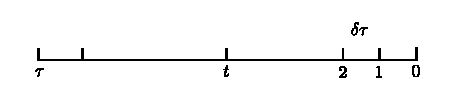
\includegraphics{Page2.pdf}
\end{wrapfigure}
Assume the initial and final configurations are $\vec{\theta}_0$, so that the path integral can be written as
\begin{equation}
    Z = \braket{\vec{\theta}_0 | e^{-\tau H/\hbar} | \vec{\theta}_0}
\end{equation}
Insert identity at integer time step, we have
\begin{equation}
    Z 
    = \left(\prod_{i, t} \int_{-\pi}^{\pi} \frac{d\theta_{i, t}}{2\pi}\right)
    \braket{\vec{\theta}_t | e^{-\delta \tau H/\hbar} | \vec{\theta}_{t-1}} 
\end{equation}
and then insert identity at half-integer time step, 
\begin{equation}
    Z 
    = \left(\prod_{i, t} \int_{-\pi}^{\pi} \frac{d\theta_{i, t}}{2\pi} \sum_{n_{i, t} \in \mathbb{Z} }\right)
    \braket{\vec{\theta}_t | \vec{n}_{t-1/2}} \braket{\vec{n}_{t-1/2}|\vec{\theta}_{t-1}}
    e^{-\delta \tau H(\vec{n}_{t-1/2}, \vec{\theta}_{t-1})}
\end{equation}
In the end, the Euclidean path integral is
\begin{equation}
    \begin{aligned}
        Z 
        &= \left(
            \prod_{i, t} \int_{-\pi}^{\pi} \frac{d\theta_{i, t}}{2\pi} 
            \sum_{n_{i, t} \in \mathbb{Z} }
            \right)\\
        & \times \exp \left[
            -i\sum_{i, t} n_{i, t-1/2} (\theta_{i, t} - \theta_{i, t-1}) 
            -\frac{\delta \tau}{\hbar} (
            \sum_{i, t} K n_{i, t-1/2}^2 
            - \sum_{\braket{ii'}, t} J \cos(\theta_{i, t-1} - \theta_{i', t-1})) 
        \right]          
    \end{aligned}
\end{equation}
% ============================================================================================
\paragraph*{c)} Map the Euclidean path integral to classical XY/Villain model.
\subparagraph*{$\bullet $}
The $n_{i, t}$ related terms in the integrand can be extracted as 
\begin{equation}
    \left(\prod_{i, t} \sum_{n_{i, t} \in \mathbb{Z} }\right) 
    \prod_{i, t} \exp \left[
        -\frac{\delta \tau}{\hbar} K n_{i, t-1/2}^2 - i n_{i, t-1/2} (\theta_{i, t} - \theta_{i, t-1}) 
    \right]
\end{equation}
Defining 
$ f(x) \equiv e^{\left[
    -\frac{\delta \tau}{\hbar} K x^2 - i x (\theta_{i, t} - \theta_{i, t-1}) 
\right]} $, 
then we have $\sum_{n \in \mathbb{Z}}f(n) = \sum_{n \in \mathbb{Z}} \int dx f(x)\delta(x-n)$, using Poisson resummation $\sum_{n \in \mathbb{Z}} \delta(x-n) = \sum_{n \in \mathbb{Z}} e^{i2\pi n x}$, we get $\sum_{n \in \mathbb{Z}}f(n) = \sum_{n \in \mathbb{Z}}\int dx f(x)e^{i2\pi n x}$, the Gaussian integral of $x$ can be carried out exactly
\begin{equation}
    \sum_{n \in \mathbb{Z}}f(n) = \sum_{m \in \mathbb{Z}}
    \int dx \exp(\left[
        -\frac{\delta \tau}{\hbar} K x^2 - i x (\theta_{i, t} - \theta_{i, t-1} - 2\pi m) \right]
    = \sum_{m \in \mathbb{Z}} C \exp(\frac{(\theta_{i, t} - \theta_{i, t-1} + 2\pi m)^2 }{4 \delta \tau K /\hbar})
\end{equation}
with constant $C = \sqrt{\frac{\pi}{\delta \tau /\hbar}}$. The last equation above has changed $ m \rightarrow -m$. 
Now the partition function for $D = d+1$ dimensional anisotropic classical XY model is
\begin{equation}
    \begin{aligned}
        Z_{XY} 
        & = \left(
            \prod_{i, t} \int_{-\pi}^{\pi} \frac{d\theta_{i, t}}{2\pi}
             \sum_{\tilde{m}_{i, t} \in \mathbb{Z} }
             \sqrt{\frac{\pi}{\delta \tau /\hbar}} \right)\\     
        & \times \exp \left[ 
                \frac{1}{4 \delta \tau K /\hbar} \sum_{i, t} 
                    (\theta_{i, t} - \theta_{i, t-1} + 2\pi \tilde{m}_{i, t})^2 
                + \frac{\delta \tau}{\hbar} J \sum_{\braket{ii'}, t} 
                    \cos(\theta_{i, t-1} - \theta_{i', t-1})
                    \right] 
    \end{aligned}
\end{equation}
and the partition function for Villain model is
\begin{equation} \label{Z_V}
    \begin{aligned}
        Z_{V} 
        &= \left(
            \prod_{i, t} 
            \int_{-\pi}^{\pi} \frac{d\theta_{i, t}}{2\pi} 
            \sum_{\tilde{m}_{i, t} \in \mathbb{Z}}
            \sum_{m_{l, t} \in \mathbb{Z}}
            \sqrt{\frac{\pi}{\delta \tau /\hbar}} 
            \right) \\
        & \times \exp \left[ 
            \frac{1}{4 \delta \tau K /\hbar} \sum_{i, t} 
                (d\tilde{\theta}_{i, t} + 2\pi \tilde{m}_{i, t})^2 
            + \frac{\delta \tau}{2\hbar} J \sum_{l, t} 
                (d\theta_{l, t-1} + 2\pi m_{l, t})^2
                \right]
    \end{aligned}
\end{equation}
where $l = \braket{ii'}$ and $ d\tilde{\theta}_{i, t} = \theta_{i, t} - \theta_{i, t-1}$.

Mapping coefficients to classical temperature, 
\begin{equation} \label{Temp_mapping}
    \begin{aligned}
        & \tilde{T}_{\tau} = 2 \delta \tau K /\hbar\\
        & \tilde{T}_{s} = \frac{\hbar}{\delta \tau J}
    \end{aligned}
\end{equation}
%--------------------------------------------------------------------------------------------
\subparagraph*{$\bullet$}
According to Fourier series expansion, 
\begin{equation}
    \exp \left[
        \frac{\delta \tau J}{\hbar} 
            \cos(d\theta_{l, t-1}) \right]
        = \sum_{j \in \mathbb{Z}} I_j(\frac{\delta \tau J}{\hbar} )
            e^{-ij(d\theta)_{l, t-1}}
\end{equation}
so that
\begin{equation}
    \begin{aligned}
        Z 
        & = \left(
            \prod_{i, t} \int_{-\pi}^{\pi} \frac{d\theta_{i, t}}{2\pi} 
            \sum_{n_{i, t} \in \mathbb{Z} }
            \sum_{j_{l, t} \in \mathbb{Z} } I_{j_{l, t}}(\frac{\delta \tau J}{\hbar})
            \right)  \\
        & \times \exp \left[ 
            -i\sum_{i, t} n_{i, t-1/2} (\theta_{i, t} - \theta_{i, t-1})
            -\frac{\delta \tau K}{\hbar} 
            \sum_{i, t} n_{i, t-1/2}^2 
            - \sum_{l, t} ij_{l, t-1}(d\theta)_{l, t-1}
        \right]
    \end{aligned}
\end{equation}
use $ \sum_l j_l (d\theta)_l = \sum_i (\nabla \cdot j)_i \theta_i $, the coefficient of $\theta_{i, t}$ is $ -i[(\nabla \cdot j)_i +(n_{i, t+1/2} - n_{i, t-1/2})]$, after integrating out $\theta_{i,t}$, we get 
\begin{equation} \label{Current_rep}
    \begin{aligned}
        Z 
        & = \left(
            \prod_{i, t}
            \sum_{n_{i, t} \in \mathbb{Z} }
            \sum_{j_{l, t} \in \mathbb{Z} } I_{j_{l, t}}(\frac{\delta \tau J}{\hbar})
            \right)   \\     
        & \times \exp \left[
            -\frac{\delta \tau K}{\hbar} 
                \sum_{i, t} n_{i, t-1/2}^2 
        \right]
        \prod_{i, t} \delta \left((\nabla \cdot j_t)_i + \frac{\partial n_i}{\partial t}\right)
    \end{aligned}
\end{equation}
The delta function indicated the current conservation
\begin{equation}
    (\nabla \cdot j_t)_i + \frac{\partial n_i}{\partial t} = 0
\end{equation} 
$n$ is the particle number, while $j$ is the current. 

% ============================================================================================
\paragraph*{d)} According to the equation (\ref{Temp_mapping}), \\
$ \bullet$ ``high T" in the classical model correspond to large $K$ and small $J$, we can neglect $J$ term and get the Hamiltonian constructed by boson number operator. Each term in the $H$ is commute with each other. So the Hamiltonian becomes classical.\\
In ``high T'' limit, focus on current representation (\ref{Current_rep}), and change imaginary time back to real time, the integrand of will oscillate strikingly as $K$ is large, so only the classical $ {n_{i, t}}$ contributes. And in current representation, $n$ is regarded as boson particle number. So ``high T'' corresponds to boson perspective classical.\\
$ \bullet$ ``low T" correspond to small $K$ and large $J$, we can neglect $K$ term and get the Hamiltonian classical. \\
In the same way, according to (\ref{Z_V}), only classical ${\theta_{i,t}}$ contributes most, while $\theta$ is interpreted as rotor angular coordinate.

% ============================================================================================
\paragraph*{e)} Using current representation, and include background $A$ and change $iA$ on the time link to $\mu$,
\begin{equation}
    \begin{aligned}
        Z 
        & = \left(
            \prod_{i, t} \int_{-\pi}^{\pi} \frac{d\theta_{i, t}}{2\pi} 
            \sum_{n_{i, t} \in \mathbb{Z} }
            \sum_{j_{l, t} \in \mathbb{Z} } I_{j_{l, t}}(\frac{\delta \tau J}{\hbar})
            \right)  \\
        & \times \exp \left[ 
            \sum_{i, t} n_{i, t-1/2} (\theta_{i, t-1} - \theta_{i, t} - q\mu)
            -\frac{\delta \tau K}{\hbar} 
            \sum_{i, t} n_{i, t-1/2}^2 
            - \sum_{l, t} ij_{l, t-1}(d\theta - qA)_{l, t-1}
        \right]
    \end{aligned}
\end{equation}
chemical potential couple to particle number in the form of $ e^{-\mu n}$. So when $\mu \uparrow$, $n \downarrow$, when $\mu \downarrow$, $n \uparrow$. Agree with intuition.




\section{Ising Model from Breaking XY Model}
\paragraph*{a)} 
Residual global symmetry: $\theta_v \rightarrow \theta_v + \alpha_v$, keep $ d\alpha_l = 0$ and $ \alpha_v = \frac{2\pi m}{n}, m = 0, 1, \dots, n-1 $. So now global symmetry becomes discrete.\\
When $n = 2$, $\alpha_v$ can only be ${0, \pi}$. Also, when $V \gg 1$, $ e^{V[\cos(n\theta_v) - 1]}$ peaks at $n\theta_v = 2\pi m, m\in \mathbb{Z}$, i.e. $\theta_v = 0, \pi $ contributes most. This setup behaves like Ising model very much.

\paragraph*{b)} 
As we see in $a)$, when $V \rightarrow +\infty $, $ e^{V[\cos(n\theta_v) - 1]}$ can be approximated by $ \sum_{m \in \mathbb{Z}} \delta (\frac{n\theta_v}{2\pi} - m)$. Using Poisson resummation, we have
\begin{equation}
    \sum_{m \in \mathbb{Z}} \delta (\frac{n\theta_v}{2\pi} - m)
    = \sum_{k_v \in \mathbb{Z}} e^{in k_v \theta_v}
\end{equation}
such that two partition function becomes equivalent.\\
When $n = 2$, sum over $k_v$, we get 
\begin{equation}
    Z = \left[ \prod_{v} \left(\sum_{\theta_v = 0, \pi}\right)\right]
    \prod_{l} \left(\delta_{d\theta_l = 0} + e^{-2/T} \delta_{d\theta_l = \pi}\right)
\end{equation}
This is exactly the same as Ising model. When $n$ is other value, $\theta_v \in \{ \frac{2\pi m}{n}, m = 0, 1, \dots, n-1\}$, and $d\theta_l \in \{ \frac{2\pi m}{n}, m = 0, 1, \dots, n-1\}$. 

\paragraph*{c)}
Using the current representation
\begin{equation} \label{2c_current}
    Z 
    = \left(
        \prod_{v} \int_{-\pi}^{\pi} \frac{d\theta_{v}}{2\pi} 
        \sum_{j_{l} \in \mathbb{Z} } I_{j_{l}}(\frac{1}{T})
        \right)
    \prod_{l} e^{-ij_l (d\theta)_l}
    \prod_{v} e^{V[\cos(n\theta_v)-1]}
\end{equation}
use Fourier series again, also with $ \sum_l j_l (d\theta)_l = \sum_v (\nabla \cdot j)_v \theta_v $, we have
\begin{equation}
    Z 
    = \left(
        \prod_{v} \int_{-\pi}^{\pi} \frac{d\theta_{v}}{2\pi} 
        \sum_{j_{l} \in \mathbb{Z} } I_{j_{l}}(\frac{1}{T})
        \sum_{k_{v} \in \mathbb{Z} } I_{k_{v}}(V)
        \right)
    \prod_{v} e^{-i (\nabla \cdot j)_v \theta_v  -ik_v n\theta_v}e^{-V}
\end{equation}
after integrating out $\theta_v$, we get $\nabla \cdot j  + nk_v = 0 $, which means current only conserved mod $n$.\\
When $n =2$, focus on equation (\ref{2c_current}), when $j_l$ is even, sum over $d \theta_l = 0, \pi $, we get $2$, but when $j_l $ is odd, alter summing over $d\theta_l$ we get zero. So only even $j$ contributes. This is the same picture of the high expansion of Ising model.

\paragraph*{d)}
$\theta_v \rightarrow \theta_v + \alpha_v$, $ A_l \rightarrow A_l + d \alpha_l$, as $ \alpha_v = \frac{2\pi m}{n}, m = 0, 1, \dots, n-1 $, $ d\alpha_l = \frac{2\pi m}{n}, m = 0, 1, \dots, n-1 $, so 
\begin{equation}
    e^{iA_l} \in \{ e^{i2\pi m /n}, m = 0, 1, \dots, n-1 \}
\end{equation}
for $n = 2$, $ e^{iA_l} = 1, -1$, corresponds to $ e^{[\pm \cos (d\theta)_l -1]/T}$, i.e. flipping the sign of the Ising couplings.
So gauge transformation  in terms of Ising model is just flip the sign of the couplings locally.